
\section{Verification}\label{sect:verif}
\optsection{Verification}

\bigskip
\begin{quote}  Two types of errors may be distinguished: modeling errors and numerical errors.  Modeling errors arise from not solving the right equations.  Numerical errors result from not solving the equations right.  The assessment of modeling errors is \emph{validation}, whereas the assessment of numerical errors is called \emph{verification} \dots  Validation makes sense only after verification, otherwise agreement between measured and computed results may well be fortuitous.
\end{quote}\index{validation versus verification}
\hfill P.~Wesseling, (2001)  \emph{Principles of Computational Fluid Dynamics}, pp.~560--561 \cite{Wesseling}
\bigskip

\subsection{Ideas}  Verification is a crucial task for a code as complicated as PISM.\index{PISM!verification of}  It is the essentially mathematical task of checking that the predictions of the numerical code are close to the predictions of the continuum model (the one which the numerical code claims to approximate).  In verification there is no comparison between model output and observations of nature.  Instead, one compares exact solutions of the continuum model, in circumstance in which they are available, to the numerical approximations of those solutions.

Reference \cite{Roache} gives a broad discussion of verification and validation in computational fluid dynamics. See \cite{BLKCB} and \cite{BBL} for discussion of verification issues for the isothermal and thermomechanically coupled shallow ice approximation (SIA), respectively, and for exact solutions to these models, and \cite{BBssasliding,SchoofStream} for verification using an exact solution to the SSA equations for ice streams.  

In PISM there is a separate executable \verb|pismv| which is used for verification.  The source codes which are verified by \verb|pismv| are, however, exactly the same, in exactly the same source files, as is run by the non-verification executables \verb|pismr|, \verb|pisms|, \verb|pgrn|, etc.  In technical terms, \verb|pismv| runs a derived class of the base class \verb|IceModel|\index{IceModel C++ class!derived class for verification}.  All PISM executables run \verb|IceModel|, but derived classes add bits of code, in this case the exact solutions.

\begin{table}[ht]
\centering
\caption{Exact solutions for verification.}\label{tab:tests}
\small
\begin{tabular}{p{0.1\linewidth}p{0.4\linewidth}p{0.25\linewidth}p{0.15\linewidth}}\hline
\textbf{Test} & \textbf{Continuum model tested} & \textbf{Comments} & \textbf{Reference} \\ \hline
A & isothermal SIA, steady,  flat bed, constant accumulation &  & \cite{BLKCB} \\
B & isothermal SIA, flat bed, zero accum & similarity soln & \cite{BLKCB,Halfar83} \\
C & isothermal SIA, flat bed, growing accum & similarity soln & \cite{BLKCB} \\
D & isothermal SIA, flat bed, oscillating accum & compensatory accum & \cite{BLKCB} \\
E & isothermal SIA; as A  but with sliding in a sector &  compensatory accum & \cite{BLKCB} \\
F & thermomechanically coupled SIA (mass and energy cons.), steady, flat bed &  compensatory accum and comp~heating& \cite{BB,BBL} \\
G & thermomechanically coupled SIA; as F  but with oscillating accumulation  & ditto & \cite{BB,BBL} \\
H & bed deformation coupled with isothermal SIA & joined similarity & \cite{BLKfastearth} \\
I & stream velocity computation using SSA (plastic till) &  & \cite{SchoofStream,BBssasliding} \\
J & shelf velocity computation using SSA  &  & [IN PREP] \\
K & pure conduction in ice and bedrock & & \cite{BuelerTestK} \\
L & isothermal SIA, steady, non-flat bed & numerical ODE soln & [IN PREP] \\
M & velocity solution for circular, constant-thickness  ice shelf with grounding line and calving front & numerical ODE soln & [NOT READY] \\
\hline
\normalsize
\end{tabular}
\end{table}

\begin{table}[ht]
  \centering
  \begin{tabular}{lp{0.7\linewidth}}
    \\\toprule
    \textbf{Option} & \textbf{Description}
    \\\midrule
    \intextoption{test} & Choose which verification test to run by giving its
    single character name; see table \ref{tab:tests}.\\
    \intextoption{no_report} & Do not report errors at the end of a verification run.\\
    \intextoption{eo} & Only evaluate the exact solution (don't do numerical
    approximation at all).
   \\\bottomrule
  \end{tabular}
  \caption{pismv command-line options}
  \label{tab:pismv-options}
\end{table}

\begin{table}[ht]
\centering
\caption{Canonical PISM\index{pismv!options to run verification tests}\index{verification tests} verification runs using the exact solutions listed in table \ref{tab:tests}.}\label{tab:tests-exec}
\small
\begin{tabular}{@{}llll}\hline
\textbf{Test} & \textbf{Example invocation}  \\ \hline
A & \verb|pismv -test A -Mx 61 -My 61 -Mz 11 -y 25000| \\
B & \verb|pismv -test B -Mx 61 -My 61 -Mz 11 -ys 422.45 -y 25000|  \\
C & \verb|pismv -test C -Mx 61 -My 61 -Mz 11 -y 15208.0|  \\
D & \verb|pismv -test D -Mx 61 -My 61 -Mz 11 -y 25000|  \\
E & \verb|pismv -test E -Mx 61 -My 61 -Mz 11 -y 25000|  \\
F & \verb|pismv -test F -Mx 61 -My 61 -Mz 61 -y 25000|  \\
G & \verb|pismv -test G -Mx 61 -My 61 -Mz 61 -y 25000|  \\
H & \verb|pismv -test H -Mx 61 -My 61 -Mz 11 -y 40034 -bed_def_iso| \\
I & \verb|pismv -test I -Mx 500 -My 5 -ssa_rtol 1e-6 -ksp_rtol 1e-11| \\
J & \verb|pismv -test J -Mx 60 -My 60 -Mz 11 -ksp_rtol 1e-12| \\
K & \verb|pismv -test K -Mx 6 -My 6 -Mz 401 -Mbz 101 -y 130000| \\
L & \verb|pismv -test L -Mx 61 -My 61 -Mz 31 -y 25000| \\
M & \emph{not ready} \\
\hline
\normalsize
\end{tabular}
\end{table}

Table \ref{tab:tests} summarizes the many exact solutions currently available in PISM.  Most of these exact solutions are solutions of \emph{free boundary problems} for partial differential equations; only Tests A, E, J, K are fixed boundary value problems.  Table \ref{tab:tests-exec} shows how to run each of them on a coarse grids.

\subsection{Refinement}  To meaningfully verify a numerical code one must go down a grid refinement path and measure numerical error for each grid \cite{Roache}.  By ``a refinement path''\index{refinement path!definition} we mean the specification of a sequence of grid cell sizes which decrease toward the refinement limit of zero size \cite{MortonMayers}.  For example, in the two spatial and one time dimension case this means a sequence of triples $(\Delta x,\Delta y,\Delta t)$ which decrease toward the unreachable continuum limit $(0,0,0)$.  By ``measuring the error for each grid'' we will mean computing a norm (or norms) of the difference between the numerical solution and the exact solution.

The goal of verification is not generally to see that the error is zero at any stage on the refinement path, or even to show that the error is small in a predetermined absolute sense.  Rather the goals are
\begin{itemize}
\item to see that the error \emph{is} decreasing,
\item to measure the rate at which it decreases, and
\item to develop a realistic sense of the magnitude of numerical error which might occur in a realistic ice sheet model run.
\end{itemize}
Knowing the error decay rate may even give a prediction of how fine a grid is necessary to achieve a desired smallness for the numerical error.

(Numerical errors are certainly not presumed to dominate among reasons why ice sheet models give imperfect results.  Other sources of ``errors'' include those from using the wrong (e.g.~over-simplified or incorrectly-parameterized) continuum model, and from observational or pre-processing errors present in input data.)

For an example of a refinement path, consider the goal of evaluating the isothermal shallow ice approximation components of PISM.  One available exact solution is the Halfar similarity solution \cite{Halfar83}, with zero accumulation, namely test B.  Here is a refinement path for evaluating numerical error relative to test B:\index{refinement path!example}\index{pismv}
\begin{quote}\small
\begin{verbatim}
pismv -test B -ys 422.45 -y 25000 -Mx 31 -My 31 -Mz 11
pismv -test B -ys 422.45 -y 25000 -Mx 61 -My 61 -Mz 11
pismv -test B -ys 422.45 -y 25000 -Mx 121 -My 121 -Mz 11
pismv -test B -ys 422.45 -y 25000 -Mx 241 -My 241 -Mz 11
\end{verbatim}
\normalsize\end{quote}
One specifies the number of grid points, but this is equivalent to specifying the grid cell sizes if the overall dimensions of the computational box is fixed; see subsection \ref{subsect:coords}.  The refinement path is the sequence of triples $(\Delta x,\Delta y,\Delta t)$ with $\Delta x = \Delta y = 80,40,20,10$ and where $\Delta t$ is determined adaptively by a stability criterion (see subsection \ref{subsect:adapt}).  Note that the vertical grid spacing $\Delta z$ is fixed because this test is isothermal and the error does not depend on changing $\Delta z$.  The above four runs produce (parts of) figures 7, 8, 9, and 10 of \cite{BLKCB}, which show that the isothermal mass conservation scheme does a reasonable job of approximating the evolving surface.  Future improvements in the numerical scheme may make the error decrease faster or be smaller.

For thermocoupled tests one refines in three dimensions.  For example, the runs\index{refinement path!example}
\begin{quote}\small
\begin{verbatim}
pismv -test G -max_dt 10.0 -y 25000 -Mx 61 -My 61 -Mz 61
pismv -test G -max_dt 10.0 -y 25000 -Mx 91 -My 91 -Mz 91
pismv -test G -max_dt 10.0 -y 25000 -Mx 121 -My 121 -Mz 121
pismv -test G -max_dt 10.0 -y 25000 -Mx 181 -My 181 -Mz 181
pismv -test G -max_dt 10.0 -y 25000 -Mx 241 -My 241 -Mz 241
pismv -test G -max_dt 10.0 -y 25000 -Mx 361 -My 361 -Mz 361
\end{verbatim}
\normalsize\end{quote}
produced figures 13, 14, and 15 of \cite{BBL}.  The last two runs, especially, require a supercomputer; the $361\times 361\times 361$ run involves more than $100$ million unknowns, updated at each of millions of time steps.  (Appropriate use \verb|-skip 10| and \verb|-z_spacing quadratic| accelerates such runs.  See subsection \ref{sec:practical-usage}.)

\subsection{Sample verification results}  Figures \ref{fig:thickerrsB} through \ref{fig:temperrsK} show a sampling of the results of verifying PISM using the tests described above.\index{PISM!verification results and reporting}  These figures were produced more-or-less automatically using Python scripts \verb|test/verifynow.py|\index{verifynow.py} and \verb|test/vnreport.py|\index{vnreport.py}.  See subsection \ref{subsect:scripts}.

It must be pointed out that, to the experienced eye, these figures \emph{do not} show outstanding rates of convergence.  For the errors in tests B and G, a partial explanation comes in the discussion of margin shape in \cite{BLKCB}, and also from presumably imperfect numerical analysis choices.  For the errors in test I, a partial explanation is low degree of smoothness present for solutions in the Sobolev space used in \cite{SchoofStream}, but again perhaps from imperfect numerical choices.  We believe, however, that the free boundary nature of the continuum problems addressed by tests B, G, and I (and most other tests, not shown) is the underlying difficulty.  Test K, as a fixed boundary problem, does a little better \cite{BuelerTestK}.

\begin{figure}[ht]
\centering
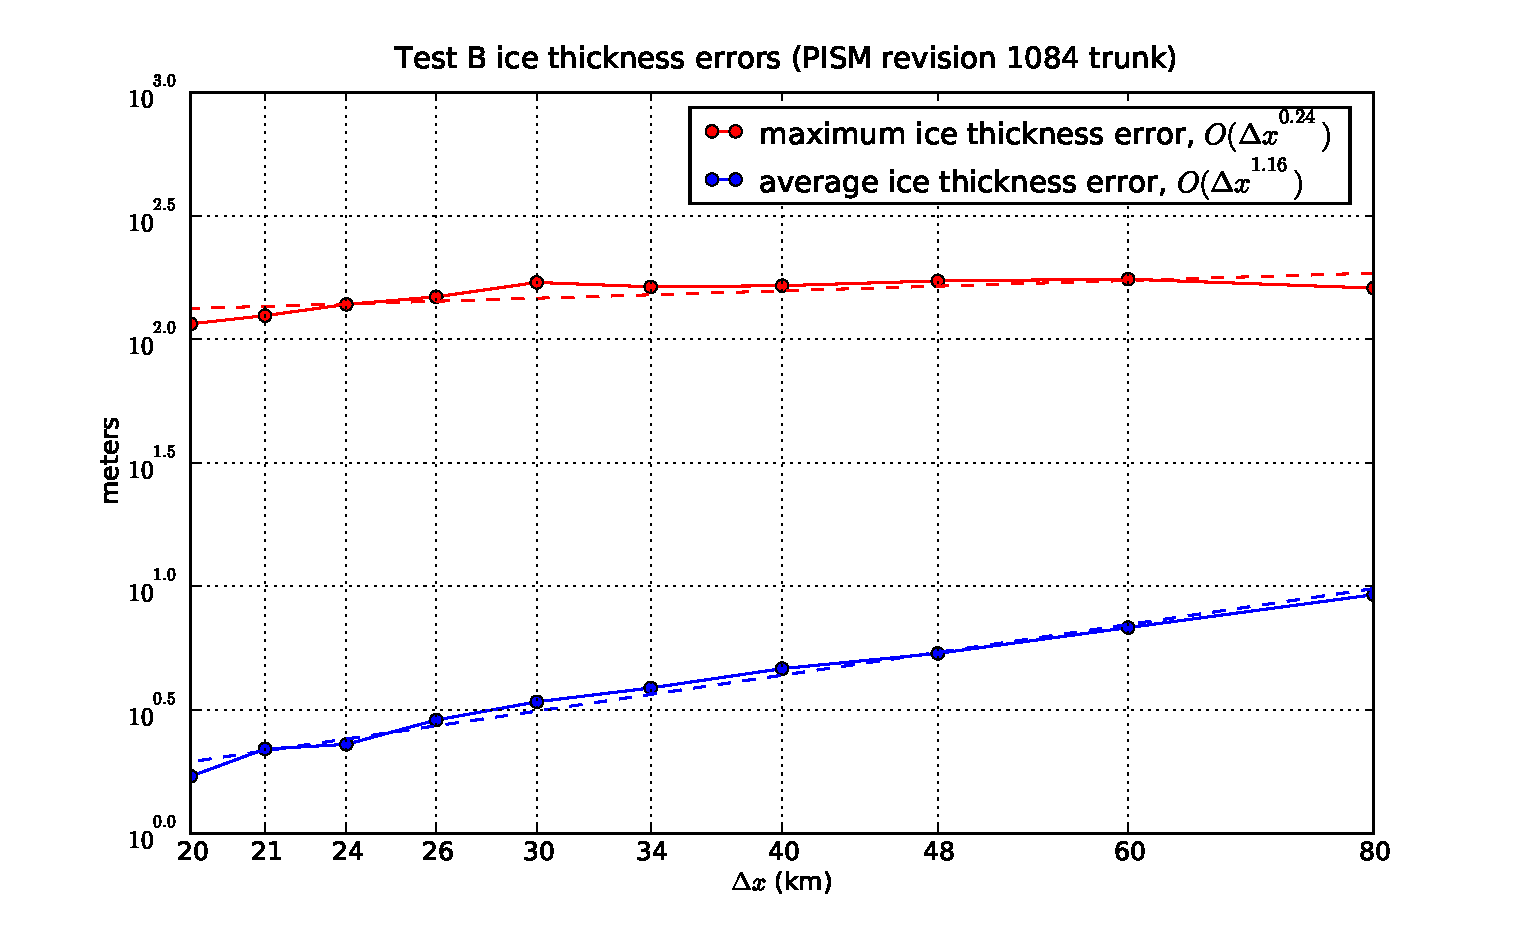
\includegraphics[width=4.8in,keepaspectratio=true]{test-B-thickness}
\caption{Numerical thickness errors in test B. See \cite{BLKCB} for discussion.}
\label{fig:thickerrsB}
\end{figure}

\begin{figure}[ht]
\centering
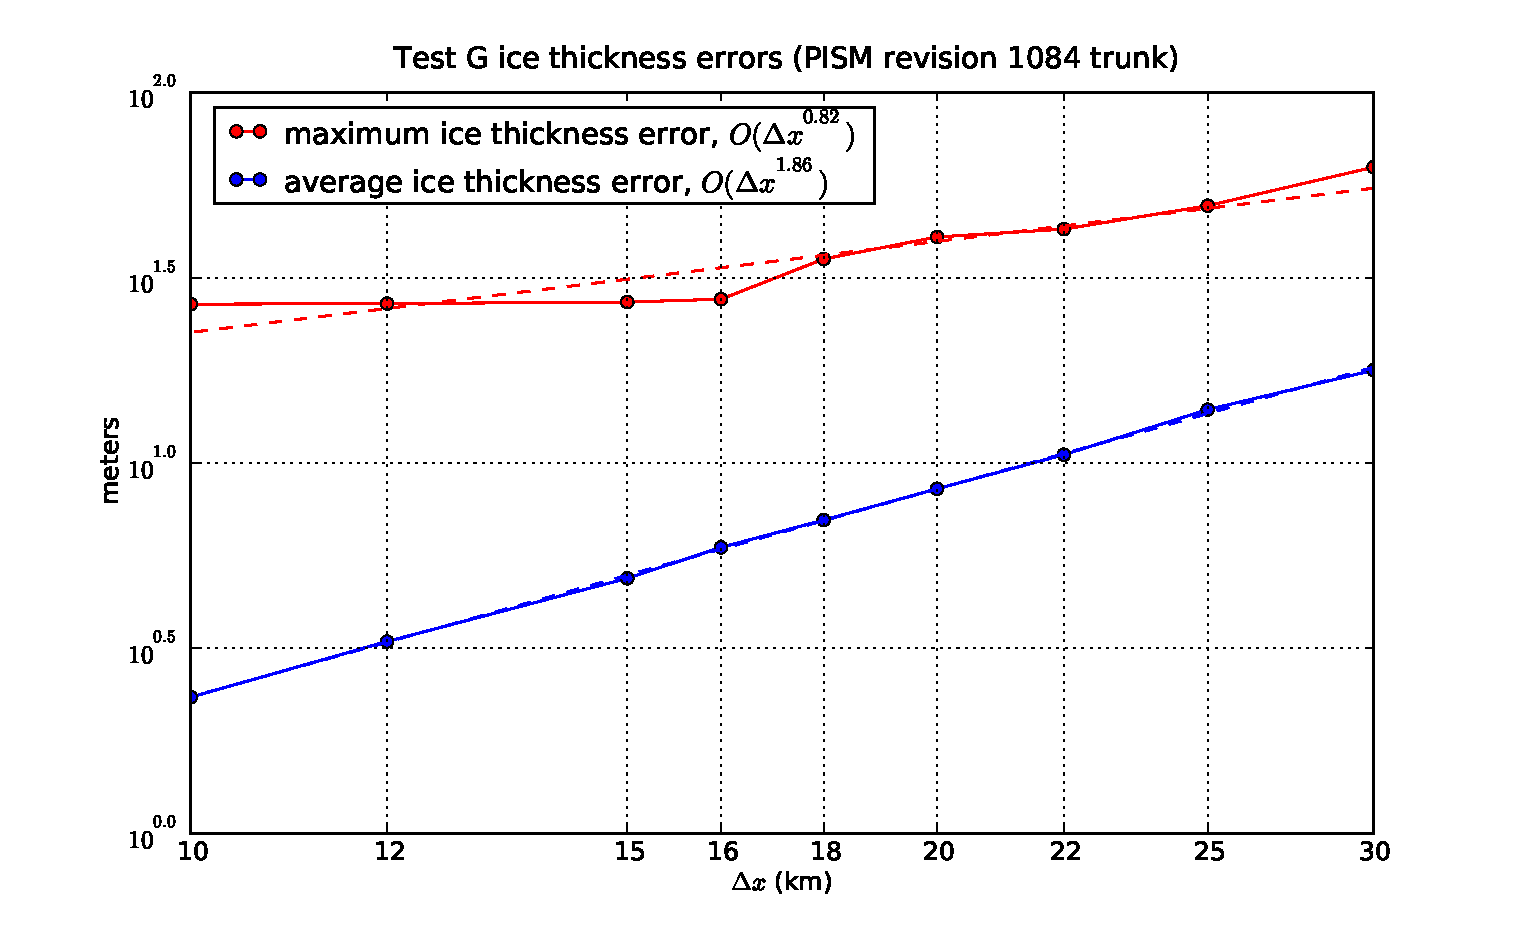
\includegraphics[width=5.0in,keepaspectratio=true]{test-G-thickness}
\caption{Numerical thickness errors in test G.  See \cite{BBL} and \cite{BLKCB}.}
\label{fig:thickerrsG}
\end{figure}

\begin{figure}[ht]
\centering
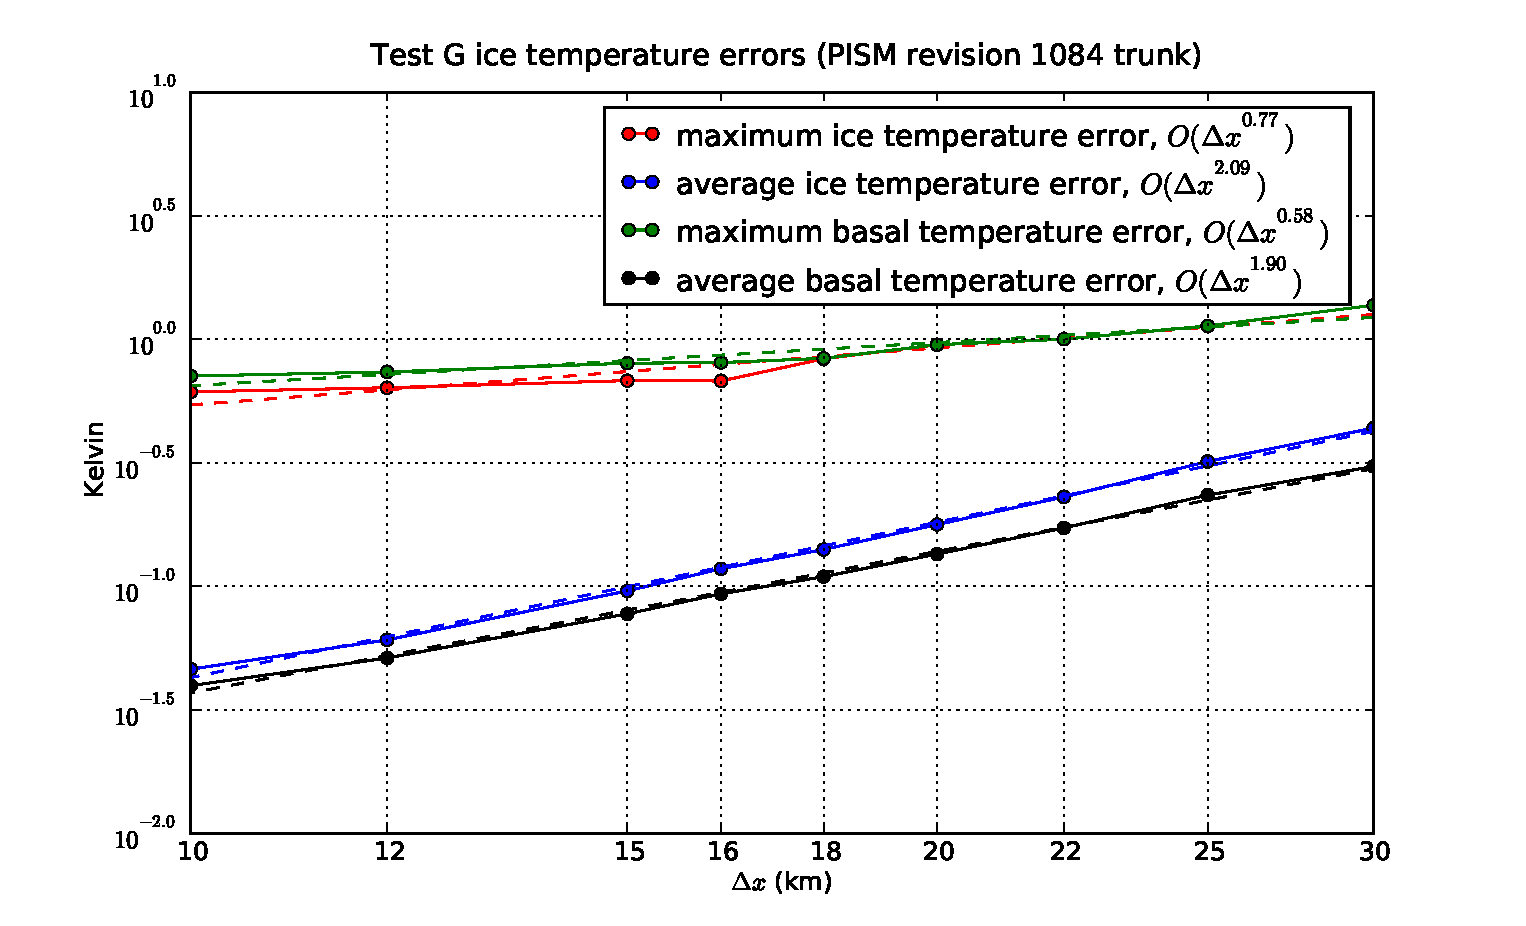
\includegraphics[width=5.0in,keepaspectratio=true]{test-G-temp}
\caption{Numerical temperature errors in test G. See \cite{BBL}.}
\label{fig:temperrsG}
\end{figure}

\begin{figure}[ht]
\centering
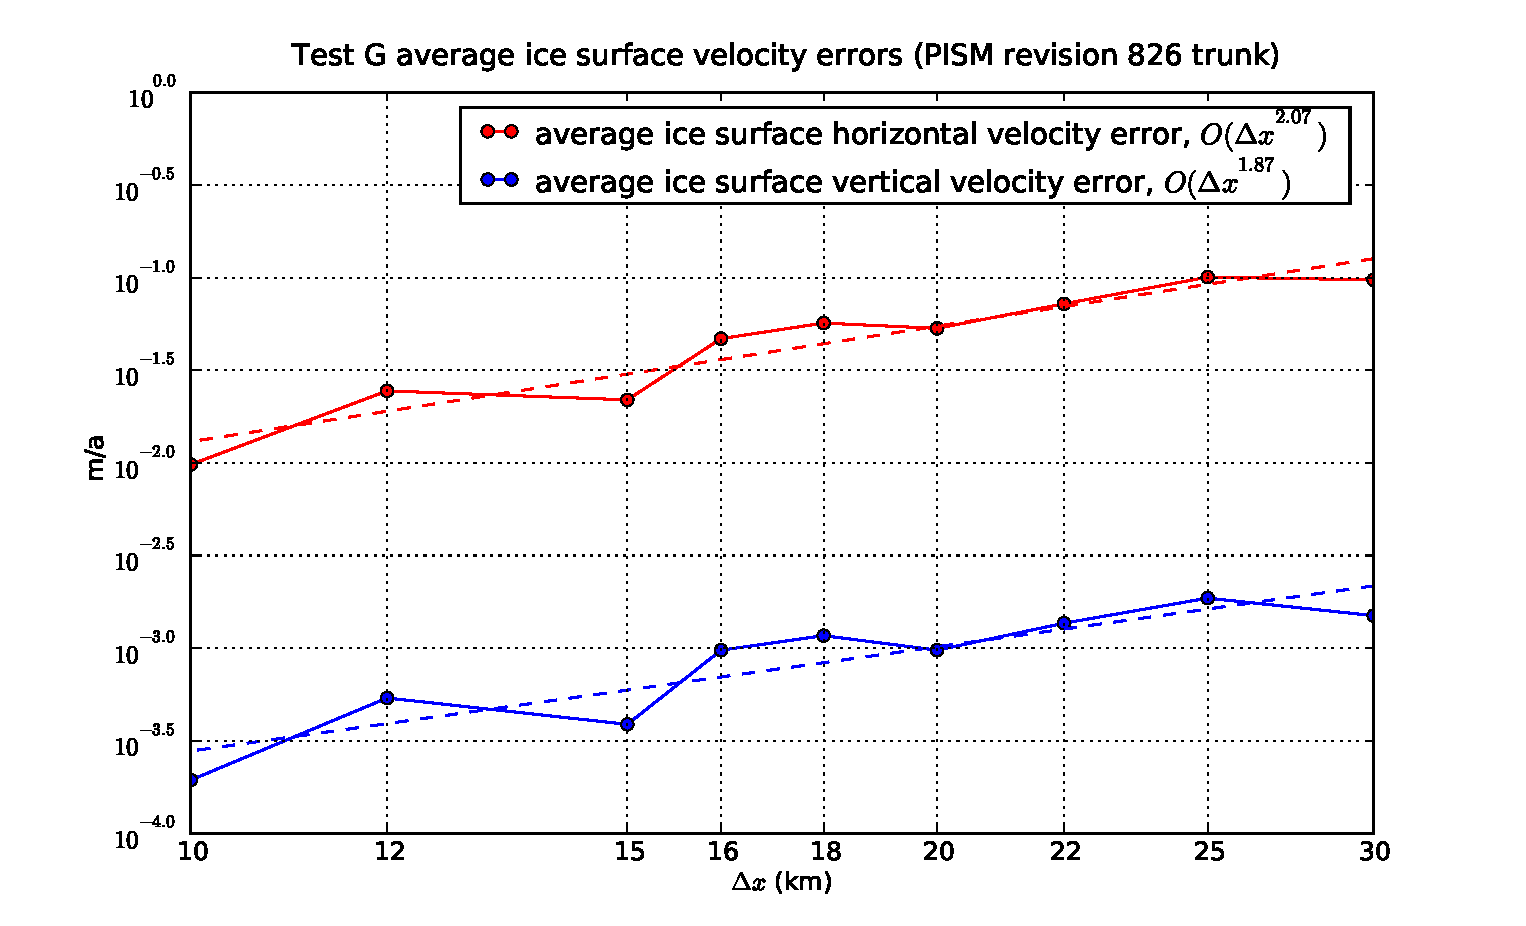
\includegraphics[width=5.0in,keepaspectratio=true]{test-G-surfvels}
\caption{Numerical errors in computed surface velocities in test G.}
\label{fig:surfvelerrsG}
\end{figure}

\begin{figure}[ht]
\centering
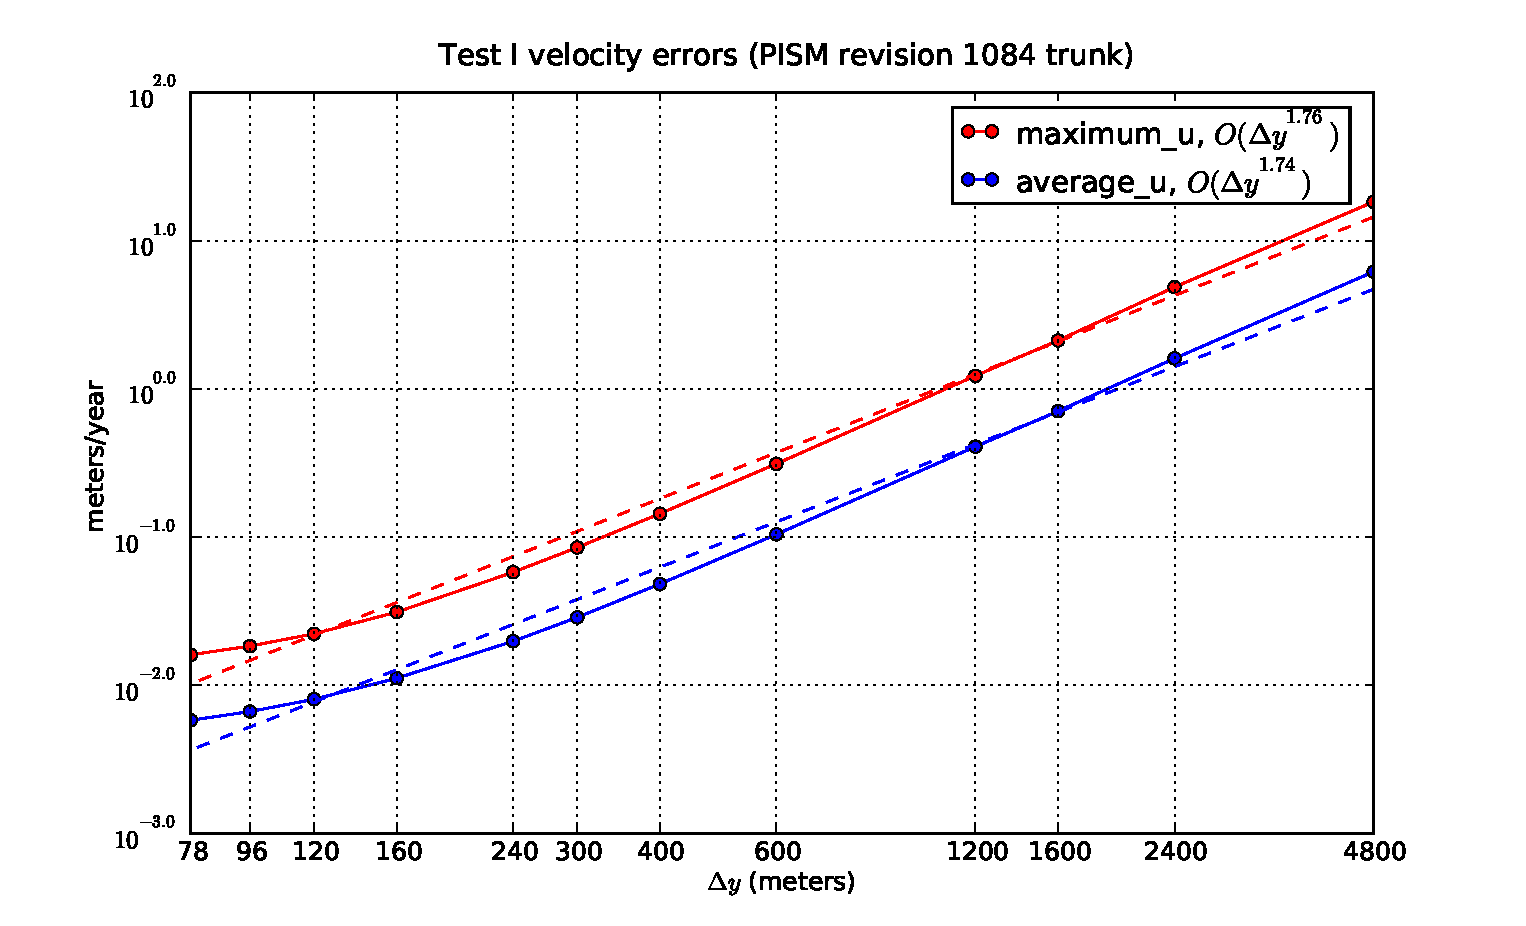
\includegraphics[width=5.0in,keepaspectratio=true]{test-I-errors}
\caption{Numerical errors in horizontal velocities in test I, an ice stream. \t{maximum_u} and \t{average_u} are errors in scalar velocity (because of symmetries in test I).  See \cite{SchoofStream,BBssasliding}.}
\label{fig:velerrsI}
\end{figure}

\begin{figure}[ht]
\centering
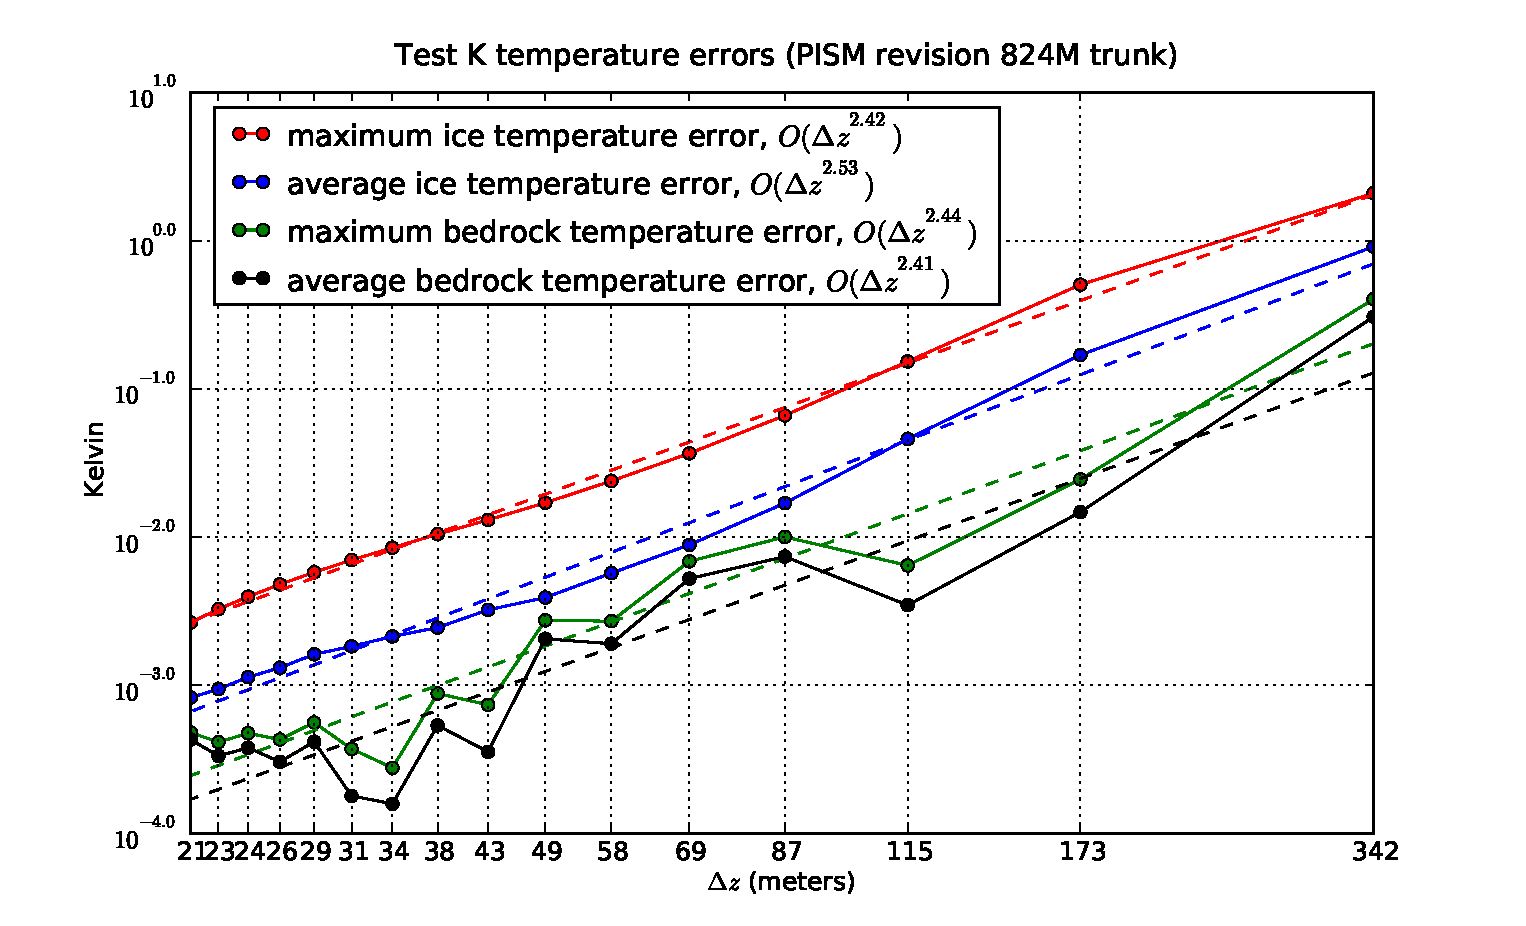
\includegraphics[width=5.0in,keepaspectratio=true]{test-K-errors}
\caption{Numerical temperature errors in test K, which tests the thermal bedrock model.  See \cite{BuelerTestK} for a discussion.}
\label{fig:temperrsK}
\end{figure}


%%% Local Variables: 
%%% mode: latex
%%% TeX-master: "manual"
%%% End: 
